\documentclass[12pt]{ctexart}

\title{测试技术课程设计报告}
\author{欧 宇恒}
\date{\today}
\usepackage{ctex}			%处理中文字体宏包
\usepackage{graphicx}		%处理图片宏包
\usepackage{amsmath}		%处理数学公式宏包	
\usepackage{setspace}		%处理行距宏包
\usepackage[left=1.91cm,right=1.91cm,top=2.54cm,bottom=2.54cm]{geometry}		%编辑页面格式
\usepackage{booktabs}		%处理三线表宏包
\usepackage{color}			%处理颜色宏包
\usepackage{multirow}       %处理合并单元格宏包
\usepackage{subfigure}
\usepackage{underscore}   % 处理下划线
\usepackage{listings} 
\usepackage{color}
\usepackage{indentfirst}
% -- Defining colors:
\usepackage[dvipsnames]{xcolor}
\definecolor{codegreen}{rgb}{0,0.6,0}
\definecolor{codegray}{rgb}{0.5,0.5,0.5}
\definecolor{codepurple}{rgb}{0.58,0,0.82}
\definecolor{backcolour}{rgb}{0.93,0.96,0.98}
\definecolor{codecolor}{rgb}{0.3,0.3,0.3}
% Definig a custom style:
\lstdefinestyle{mystyle}{
    backgroundcolor=\color{backcolour},   
    commentstyle=\color{codepurple},
    keywordstyle=\color{NavyBlue},
    numberstyle=\tiny\color{codegray},
    stringstyle=\color{codepurple},
    basicstyle=\ttfamily\footnotesize\bfseries\color{codecolor},
    breakatwhitespace=false,         
    breaklines=true,                 
    captionpos=t,                    
    keepspaces=true,                 
    numbers=left,                    
    numbersep=5pt,                  
    showspaces=false,                
    showstringspaces=false,
    showtabs=false,                  
    tabsize=2,
    frameround = ffff
}
% -- Setting up the custom style:
\lstset{style=mystyle, 
    language=python,}




\begin{document}
\ctexset{
  section={
    name={\S},
    nameformat={\zihao{3}},
    titleformat={\centering\heiti\zihao{3}},
   },
  subsection={
      name={},
      nameformat={\zihao{4}},
      titleformat={\zihao{4}},
    },
}
\begin{titlepage}

  \begin{center}
    % Upper part of the page
    
\includegraphics[width=0.4\textwidth]{./CSU.png}\\[1cm]
    \textsc{\LARGE Central South University}\\[1.5cm]
    \textsc{\Large Final Week Project}\\[1.5cm]
    % Title
    \textsc{\huge \bfseries 测试技术课程设计报告}\\[1cm]
    \textsc{\zihao{3} \bfseries 虚拟信号发生器报告}\\[1.5cm]
    % Author and supervisor
    \begin{minipage}{0.4\textwidth}
      \begin{flushleft} \large
        \emph{Author:}\\
        ***
      \end{flushleft}
    \end{minipage}
    \begin{minipage}{0.4\textwidth}
      \begin{flushright} \large
        \emph{Supervisor:} \\
        Dr.Xiao \textsc{Yougang}
      \end{flushright}
    \end{minipage}
    \vfill
    % Bottom of the page
    {\large \today}
  \end{center}
\end{titlepage}
\newpage
\tableofcontents
\newpage

\section{课程设计要求}

利用 APPDesign 设计一项虚拟信号发生器,支持生成正余弦信号、方波信号、三角波信号、随机信号等,并支持合成任意信号,对合成信号进行时域、频域、时差域、幅值域分析。

\section{研究背景}
信号发生器仿真研究是指通过计算机模拟仿真的方式,对信号发生器的工作原理、性能特性和设计参数进行研究和分析。信号发生器仿真模拟是电子工程、通信工程以及相关领域的重要一环。

1.理论实践结合:信号发生器仿真模拟为学生提供了将理论知识与实际应用相结合的机会。通过仿真软件,学生可以直观地理解信号发生器的工作原理、电路结构和参数设置,加深对课堂学习内容的理解。

2.实验室替代:信号发生器仿真模拟可以作为实验室实验的替代方案,学生可以通过仿真软件进行虚拟实验,完成与实际实验相似的操作和任务,提高实验能力和技能。

3.自主学习和探索:仿真软件提供了一个自主学习和探索的平台,学生可以根据自己的兴趣和需求,在虚拟环境中进行实验设计、参数调整和性能分析,培养自主学习和问题解决能力。

4.跨学科整合:信号发生器仿真模拟涉及到电子、通信、计算机等多个学科领域的知识,可以促进跨学科的整合和交叉学习。学生可以通过仿真实验,了解不同学科领域的应用场景和相互关联,拓展学科视野和思维方式。

5.实践应用能力培养:仿真模拟可以帮助学生培养实践应用能力,提高问题解决和工程设计能力。通过设计和仿真不同类型的信号发生器,学生可以深入了解电路设计和性能分析的方法,为将来从事相关工程和科研工作打下坚实基础。

信号发生器仿真研究在工程领域具有重要的意义,可以推动技术的发展和应用,提高系统性能和工作效率,通过对信号发生器进行仿真模拟,可以深入理解信号发生器的原理和工作特性,提高实验能力和问题解决能力。

基于此背景,我们小组进行了信号发生器的仿真研究。

\section{系统设计思路}

通过分析项目需求,本项目通过 Python 的 CustomTkinter 库建立了前端 GUI 架构与所需控件,设计后端算法调用前端框架中的变量值,绘制信号处理的仿真曲线,计算系统快速性与准确性指标。相较于 MATLAB 提供 Appdesign 框架,Python 的 CustomTkinter 库控件更为美观、易用,并且由 Python 构建出的 GUI 框架能以较小的体积打包成 .exe 文件,便于用户使用访问,综合各方面考虑,本次课程设计采用了 Python 作为编程语言。

\subsection{前端 GUI 框架设计}

虚拟随机信号发生器能够产生稳定的随机或伪随机信号,可以方便的模拟各种情况下不同特征的信号,包括模拟实际工作中的噪声等,帮助用户测定设备系统性能及动态特性、实验仿真学习等。本项目在设计时,根据项目需求与功能需要,设计前端 GUI 框架如图\ref{figure1}所示,方便后续程序开发。前端 GUI 框架设计共分为信号发生区、信号合成区、信号分析区三个部分,其中信号发生区用于发生信号的选择和调参、信号合成区用于合成信号的添加与删除、信号分析区支持对任意合成信号进行时域、频域、幅值域、时差域分析。

\begin{figure}[htbp]
  \centering
  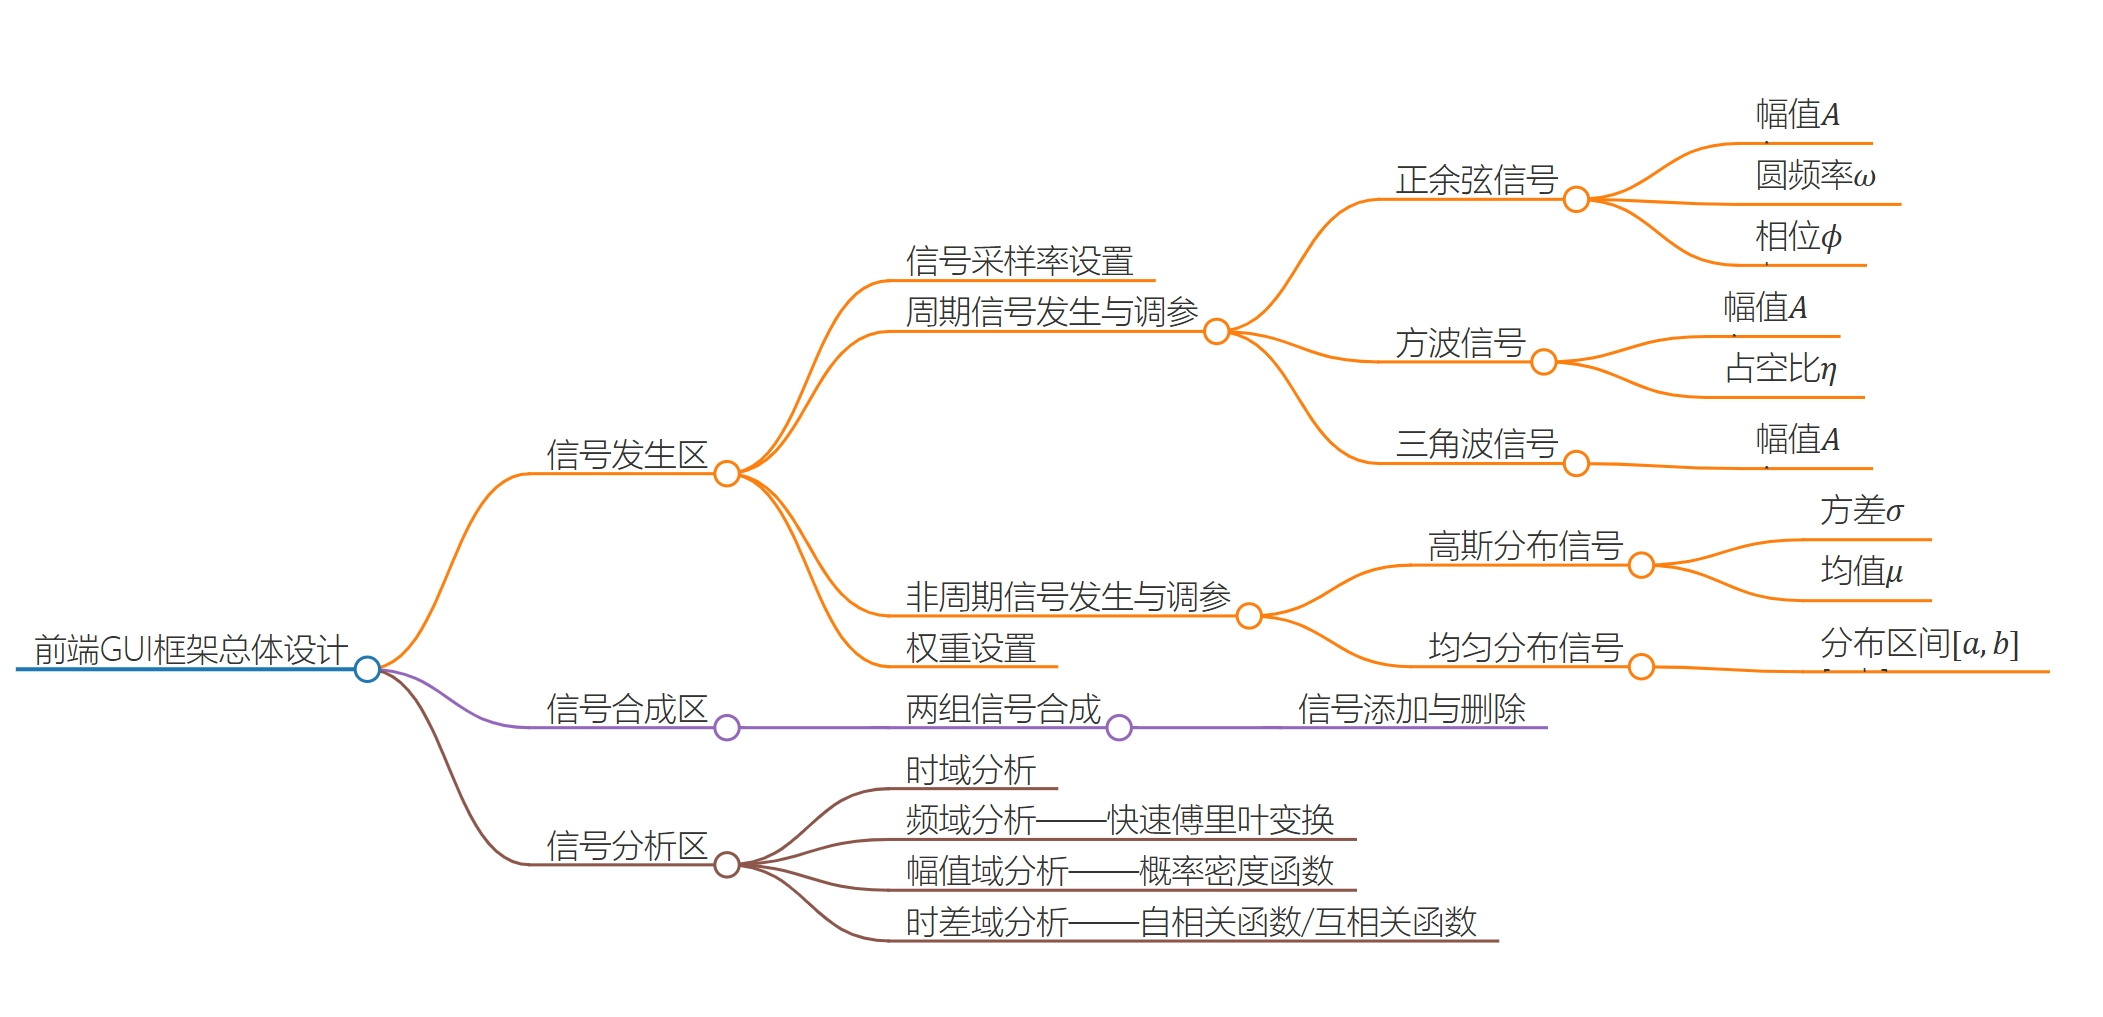
\includegraphics[width=\textwidth]{img/major_framework.png}
  \caption{前端 GUI 框架设计总思路}\label{figure1}
\end{figure}

\subsubsection{周期信号发生器}
信号的也分为周期信号与非周期信号,根据不同的设计要求选择响应的组成信号。对于周期信号发生器模块,用于生成具有固定周期和频率的电信号。可以在最上面一栏选择要生成的周期信号类型,包括方波、三角波、正弦波和矩形波等,然后调节输出信号的幅值、频率、相位和占空比等信息,得出相应的周期信号,适应不同的实验要求。周期信号发生器如图\ref{figure7}所示。
\begin{figure}[t]
  \centering
  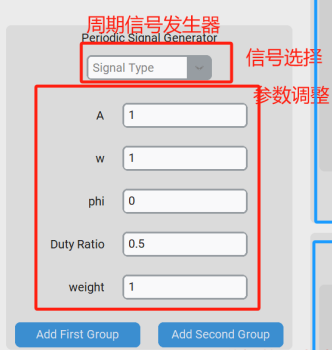
\includegraphics[width=0.3\textwidth]{img/Periodic_signal_genarator.png}
  \caption{周期信号发生器}\label{figure7}
\end{figure}

\subsubsection{随机信号发生器}
对于随机信号发生器模块,可以生成不具有固定周期和频率的电信号,其输出信号是变化的、随机的或按特定规则非周期变化。可以在最上面一栏选择要生成的非周期信号种类,包括高斯分布和均匀分布的噪声信号等,然后调节输出信号的上下限以及所占权重后,便可以输入到后续叠加模块中合成复杂信号。

\begin{figure}[t]
  \centering
  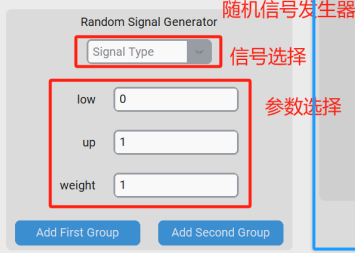
\includegraphics[width=0.3\textwidth]{img/random_signal_genarator.png}
  \caption{随机信号发生器}\label{figure8}
\end{figure}

\subsubsection{信号组合器}
信号组合器是信号发生器的重要功能之一,允许用户将多个不同类型的信号组合成一个复合信号,能够模拟复杂的信号环境。该模块将两个或多个不同频率、幅度、相位或波形的信号通过加法、乘法、调制等方式组合在一起形成一个新的信号。
在初步生成信号后便可将信号根据输入的不同权重比存入对应两组信号中,对每组信号组合处理得出对应两组信号,同时支持删除每组信号中的单一组成信号。
\begin{figure}[h]
  \centering
  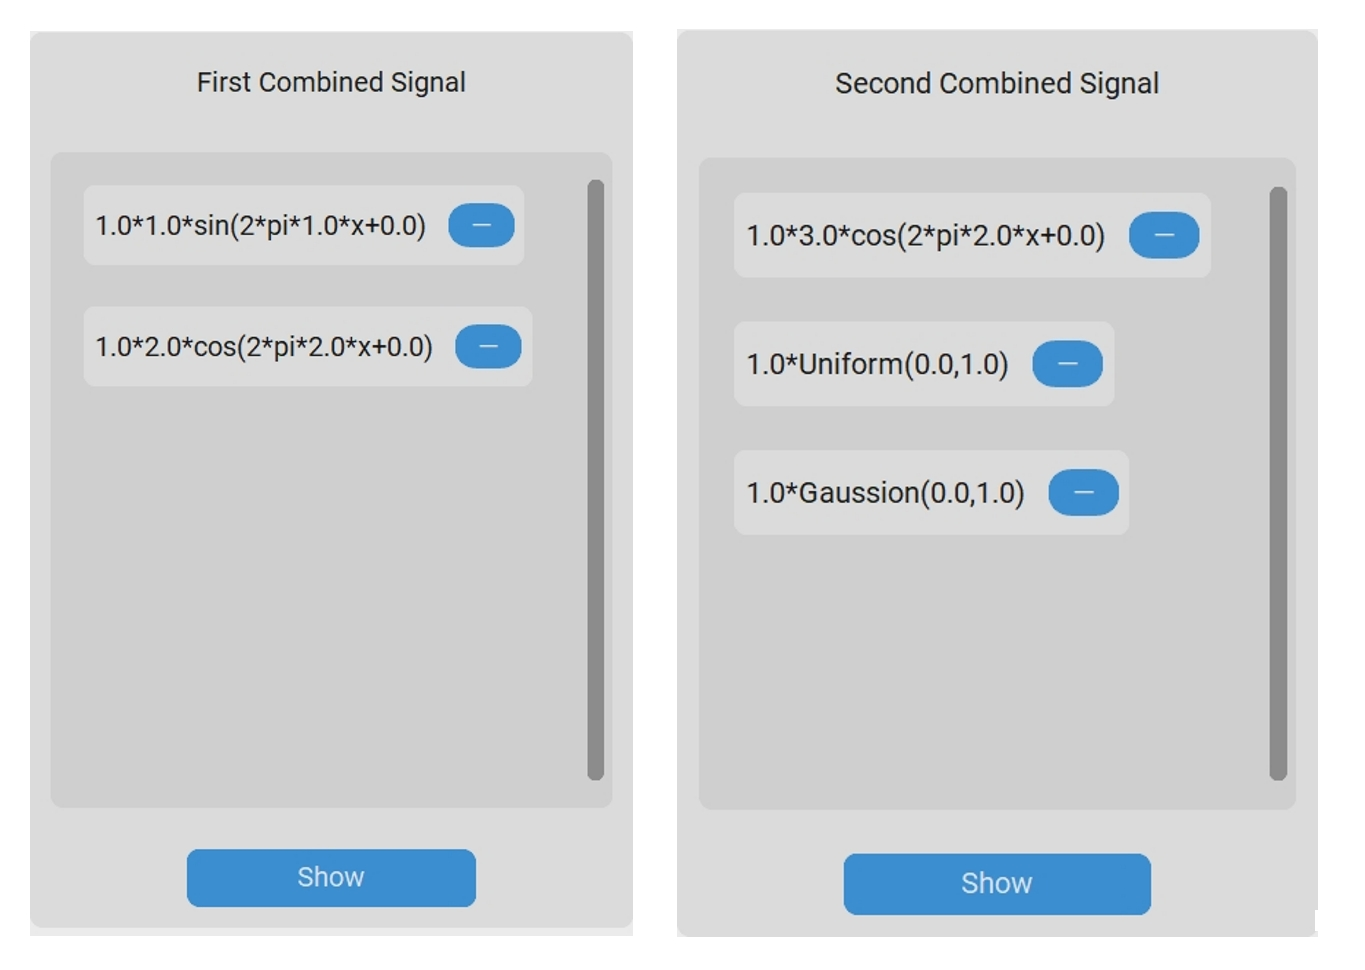
\includegraphics[width=0.5\textwidth]{img/combine_signal.png}
  \caption{信号组合器}\label{figure9}
\end{figure}


\subsection{后端算法设计}

\subsubsection{信号时间与采样率设置}

由于计算机无法存储连续数据,故数据产生时需要规定产生信号的时间与采样率,程序界面为时间和采样率的设置提供了接口,如图\ref{figure2}所示。
\begin{figure}[h]
  \centering
  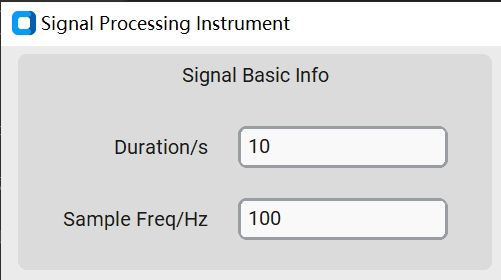
\includegraphics[width=0.3\textwidth]{img/signal_basic_info.png}
  \caption{信号采样时间与采样率设置}\label{figure2}
\end{figure}


\subsubsection{傅里叶变换}

通过傅里叶变换可以求出信号的频域,将信号分解为各个不同正余弦函数的组合,由于计算机内存储信号为离散值,此处采用离散傅里叶变换求解傅里叶级数。

在有限区间上,凡是满足狄里赫利条件的周期函数(信号)$x(t)$均能展开成傅里叶级数。傅里叶级数的三角函数展开式如下:

\begin{equation}
  x(t)=a_0+\sum_{n=1}^\infty \left(a_n \cos n\omega_0t+b_n\sin n\omega_0t\right)
\end{equation}

\begin{equation}
  \renewcommand\arraystretch{2}
  \left.\begin{matrix}
    \text{式中,常值分量} & a_0=\frac{1}{T_0}\int_{-\frac{T_0}{2}}^{\frac{T_0}{2}}x(t)dt                \\
    \text{余弦分量的幅值} & a_n=\frac{2}{T_0}\int_{-\frac{T_0}{2}}^{\frac{T_0}{2}}x(t)\cos n\omega_0tdt \\
    \text{正弦分量的幅值} & b_n=\frac{2}{T_0}\int_{-\frac{T_0}{2}}^{\frac{T_0}{2}}x(t)\sin n\omega_0tdt \\
  \end{matrix}\right\}
\end{equation}
其中,$T_0$为周期、$\omega_0$为圆频率,$\displaystyle \omega_0=\frac{2\pi}{T_0}$、$n=1,2,3,\cdots$

可以看出,周期性信号是由一个或几个、乃至无穷多个不同频率的谐波叠加而成,以圆频率作为横坐标,幅值$A_n$和相角$\phi_n$为纵坐标作图,则分别得到其幅频谱和相频谱图。由于$n$是整数序列,各频率成分都是$\omega_0$的整倍数,相邻频率的间隔$\Delta \omega=\omega_0=2\pi/T_0$,因而谱线是离散的。通常把$\omega_0$称为基频,并把成分$A_n\sin(n\omega_0t+\phi_n)$称为$n$次谐波。

本项目通过信号生成器生成一个单位幅值的三角波,并对其进行频域分析结果如图\ref{figure3}所示。可以看出,这与理论推导结果符合地较好,三角波信号的傅里叶级数为:
\begin{equation}
  x(t)=\frac{A}{2} + \frac{4A}{\pi^2}\sum_{n=1}^{\infty}\frac{1}{n^2}\cos n\omega_0t (n=1,3,5,\cdots)
\end{equation}
其幅频谱只包含常值分量、基波和奇次谐波的频率分量,谐波的幅值以$\displaystyle \frac{1}{n^2}$的规律收敛。在其相频谱中,基波和各次谐波的初相位为$\phi_n$,均为 0.

\begin{figure}[htbp]
  \centering
  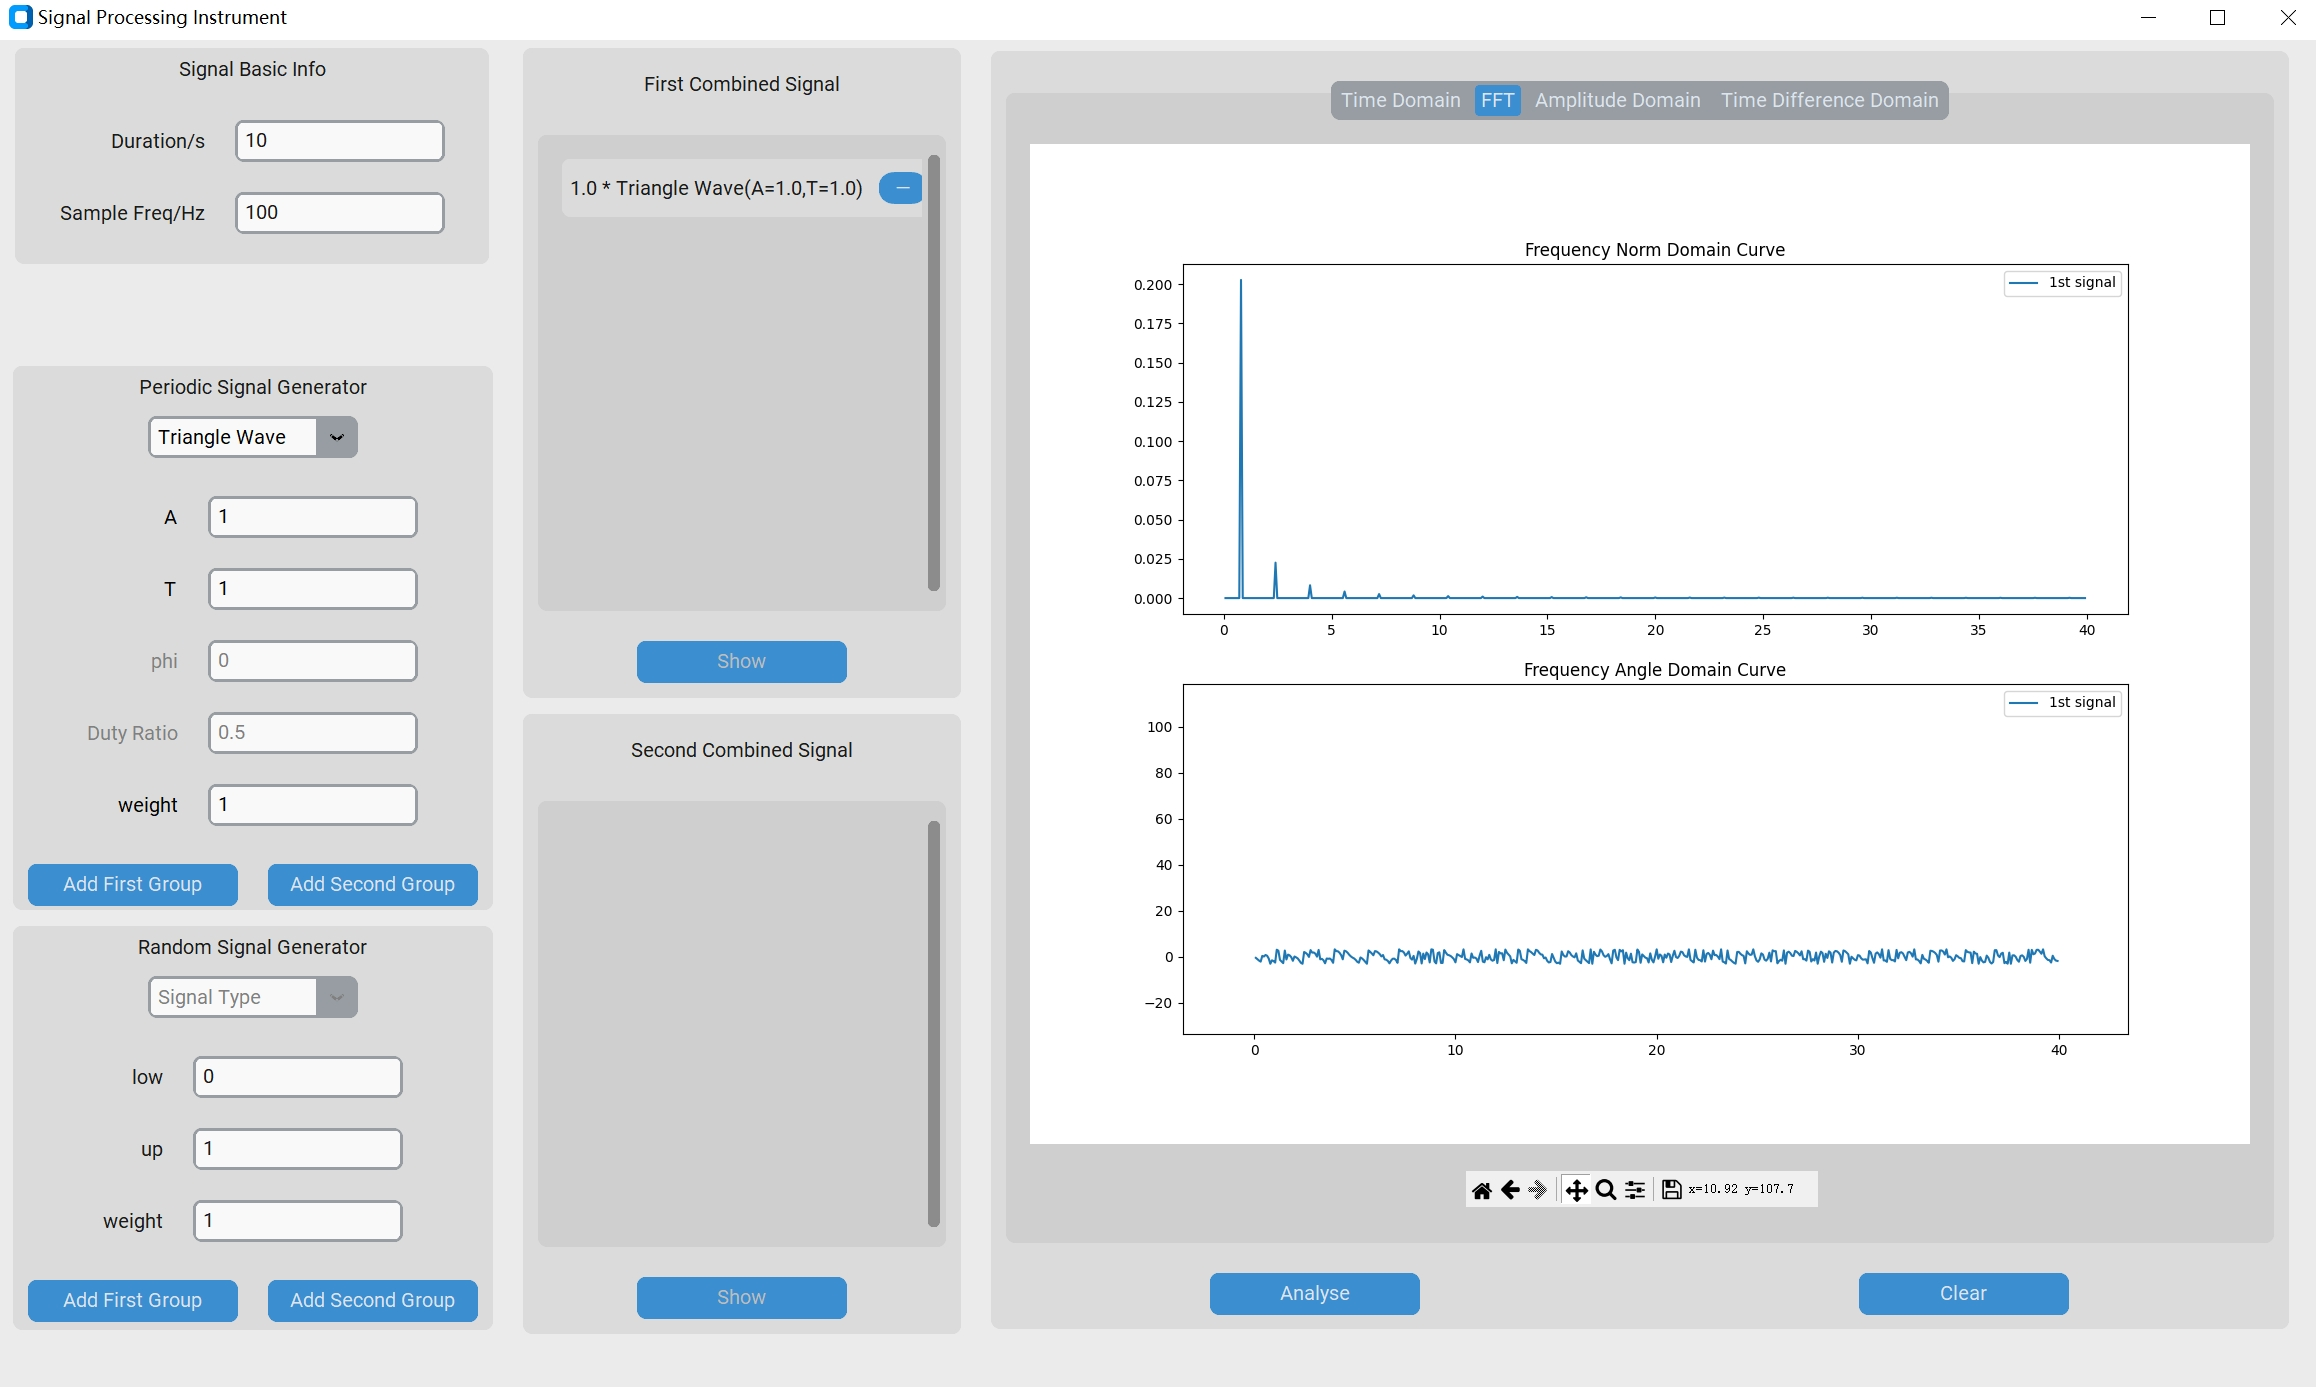
\includegraphics[width=0.9\textwidth]{img/triangle_wave_fft.png}
  \caption{单位幅值三角波频谱分析}\label{figure3}
\end{figure}

\subsubsection{幅值域分析}

幅值域分析是计算随机信号的概率密度函数,表示信号幅值落在指定区间内的概率,其具体原理如图\ref{figure4}所示。
\begin{figure}[htbp]
  \centering
  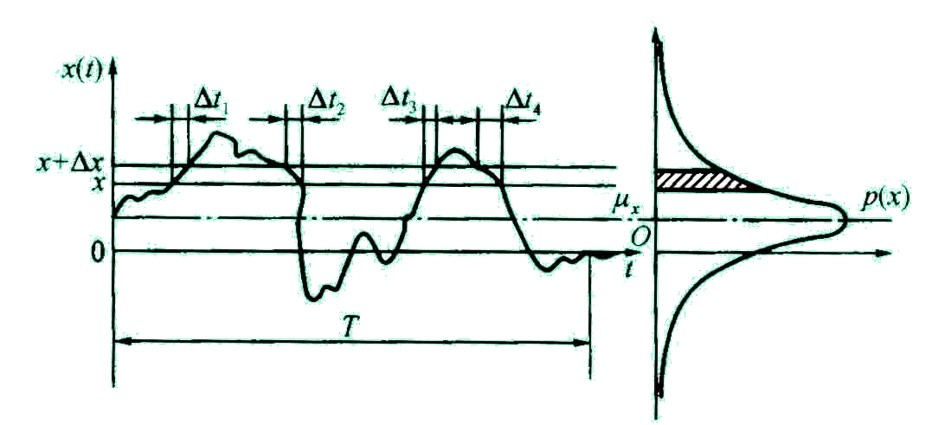
\includegraphics[width=0.5\textwidth]{img/amplitude_analysis.jpg}
  \caption{幅值域分析原理简图}\label{figure4}
\end{figure}
可以定义幅值概率密度函数$p(x)$为
\begin{equation}
  p(x)=\lim_{\Delta x\rightarrow 0}\frac{P_r\left[x<x(t)\le x+\Delta x\right]}{\Delta x}
\end{equation}
概率密度函数提供了随机信号幅值分布的信息,是随机信号的主要特征参数之一。不同的随机信号有不同的概率密度函数图像,可以借此来识别信号的性质。本项目生成了高斯分布的随机信号与正弦信号,通过幅值域分析得到结果如图\ref{figure5}所示,可以看出其与理论分析结果一致。
\begin{figure}[htbp]
  \centering
  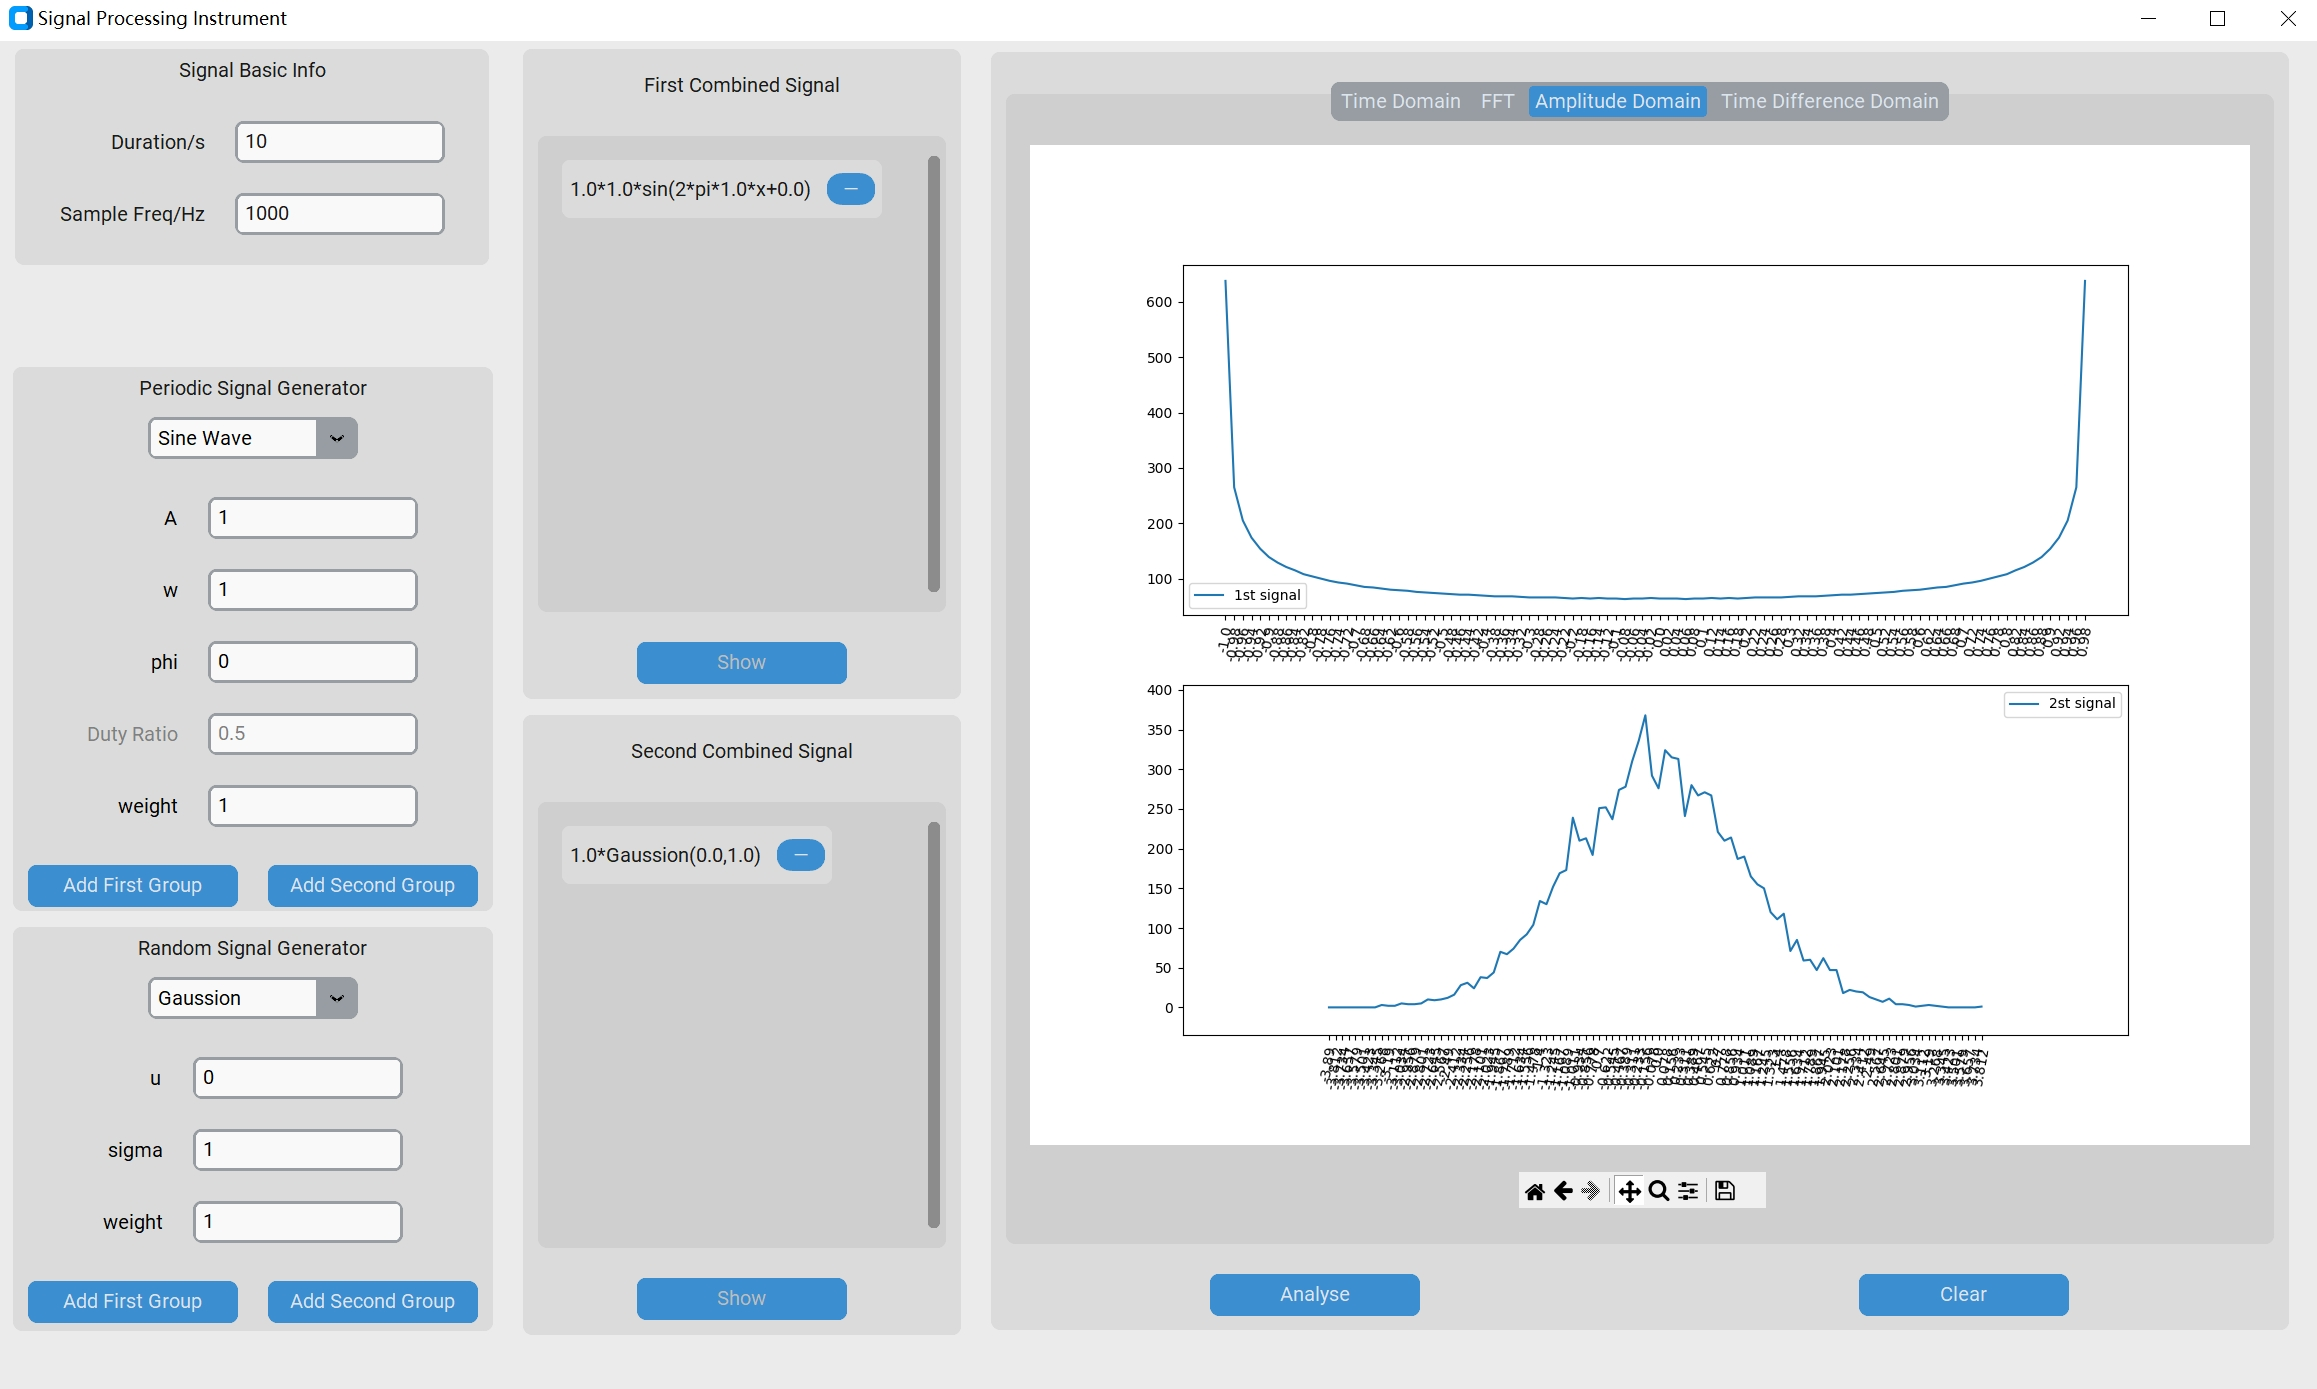
\includegraphics[width=0.9\textwidth]{img/sin_gaussion_amplitude.png}
  \caption{正弦信号与高斯分布的随机信号的幅值域分析结果}\label{figure5}
\end{figure}

\subsubsection{时差域分析}

假如$x{t}$是某各态历经随机过程的一个样本记录,$x(t+\tau)$是$x(t)$时移$\tau$后的样本,在任何$t=t_i$时刻,从两个样本上可以分别得到两个值$x(t_i)$和$x(t_i+\tau)$,而且$x(t)$和$x(t+\tau)$具有相同的均值和标准差。例如把$\rho_{x(x)x(t+\tau)}$简写作$\rho_x(\tau)$,那么有
\begin{equation}
  \rho_x(\tau)=\frac{\lim_{T\rightarrow \infty}\frac{1}{T}\int_0^T\left[x(t)-\mu_x\right]\left[x(t+\tau)-\mu_x\right]dt}{\sigma_x^2}
\end{equation}
则可以定义自相关函数$R_x(\tau)$为
\begin{equation}
  R_x(\tau)=\lim_{T\rightarrow \infty}\frac{1}{T}\int_0^Tx(t)x(t+\tau)dt
\end{equation}
本项目生成了正弦信号,通过时差域分析得到结果如图\ref{figure6}所示,可以看出其与理论分析结果一致。
\begin{figure}[htbp]
  \centering
  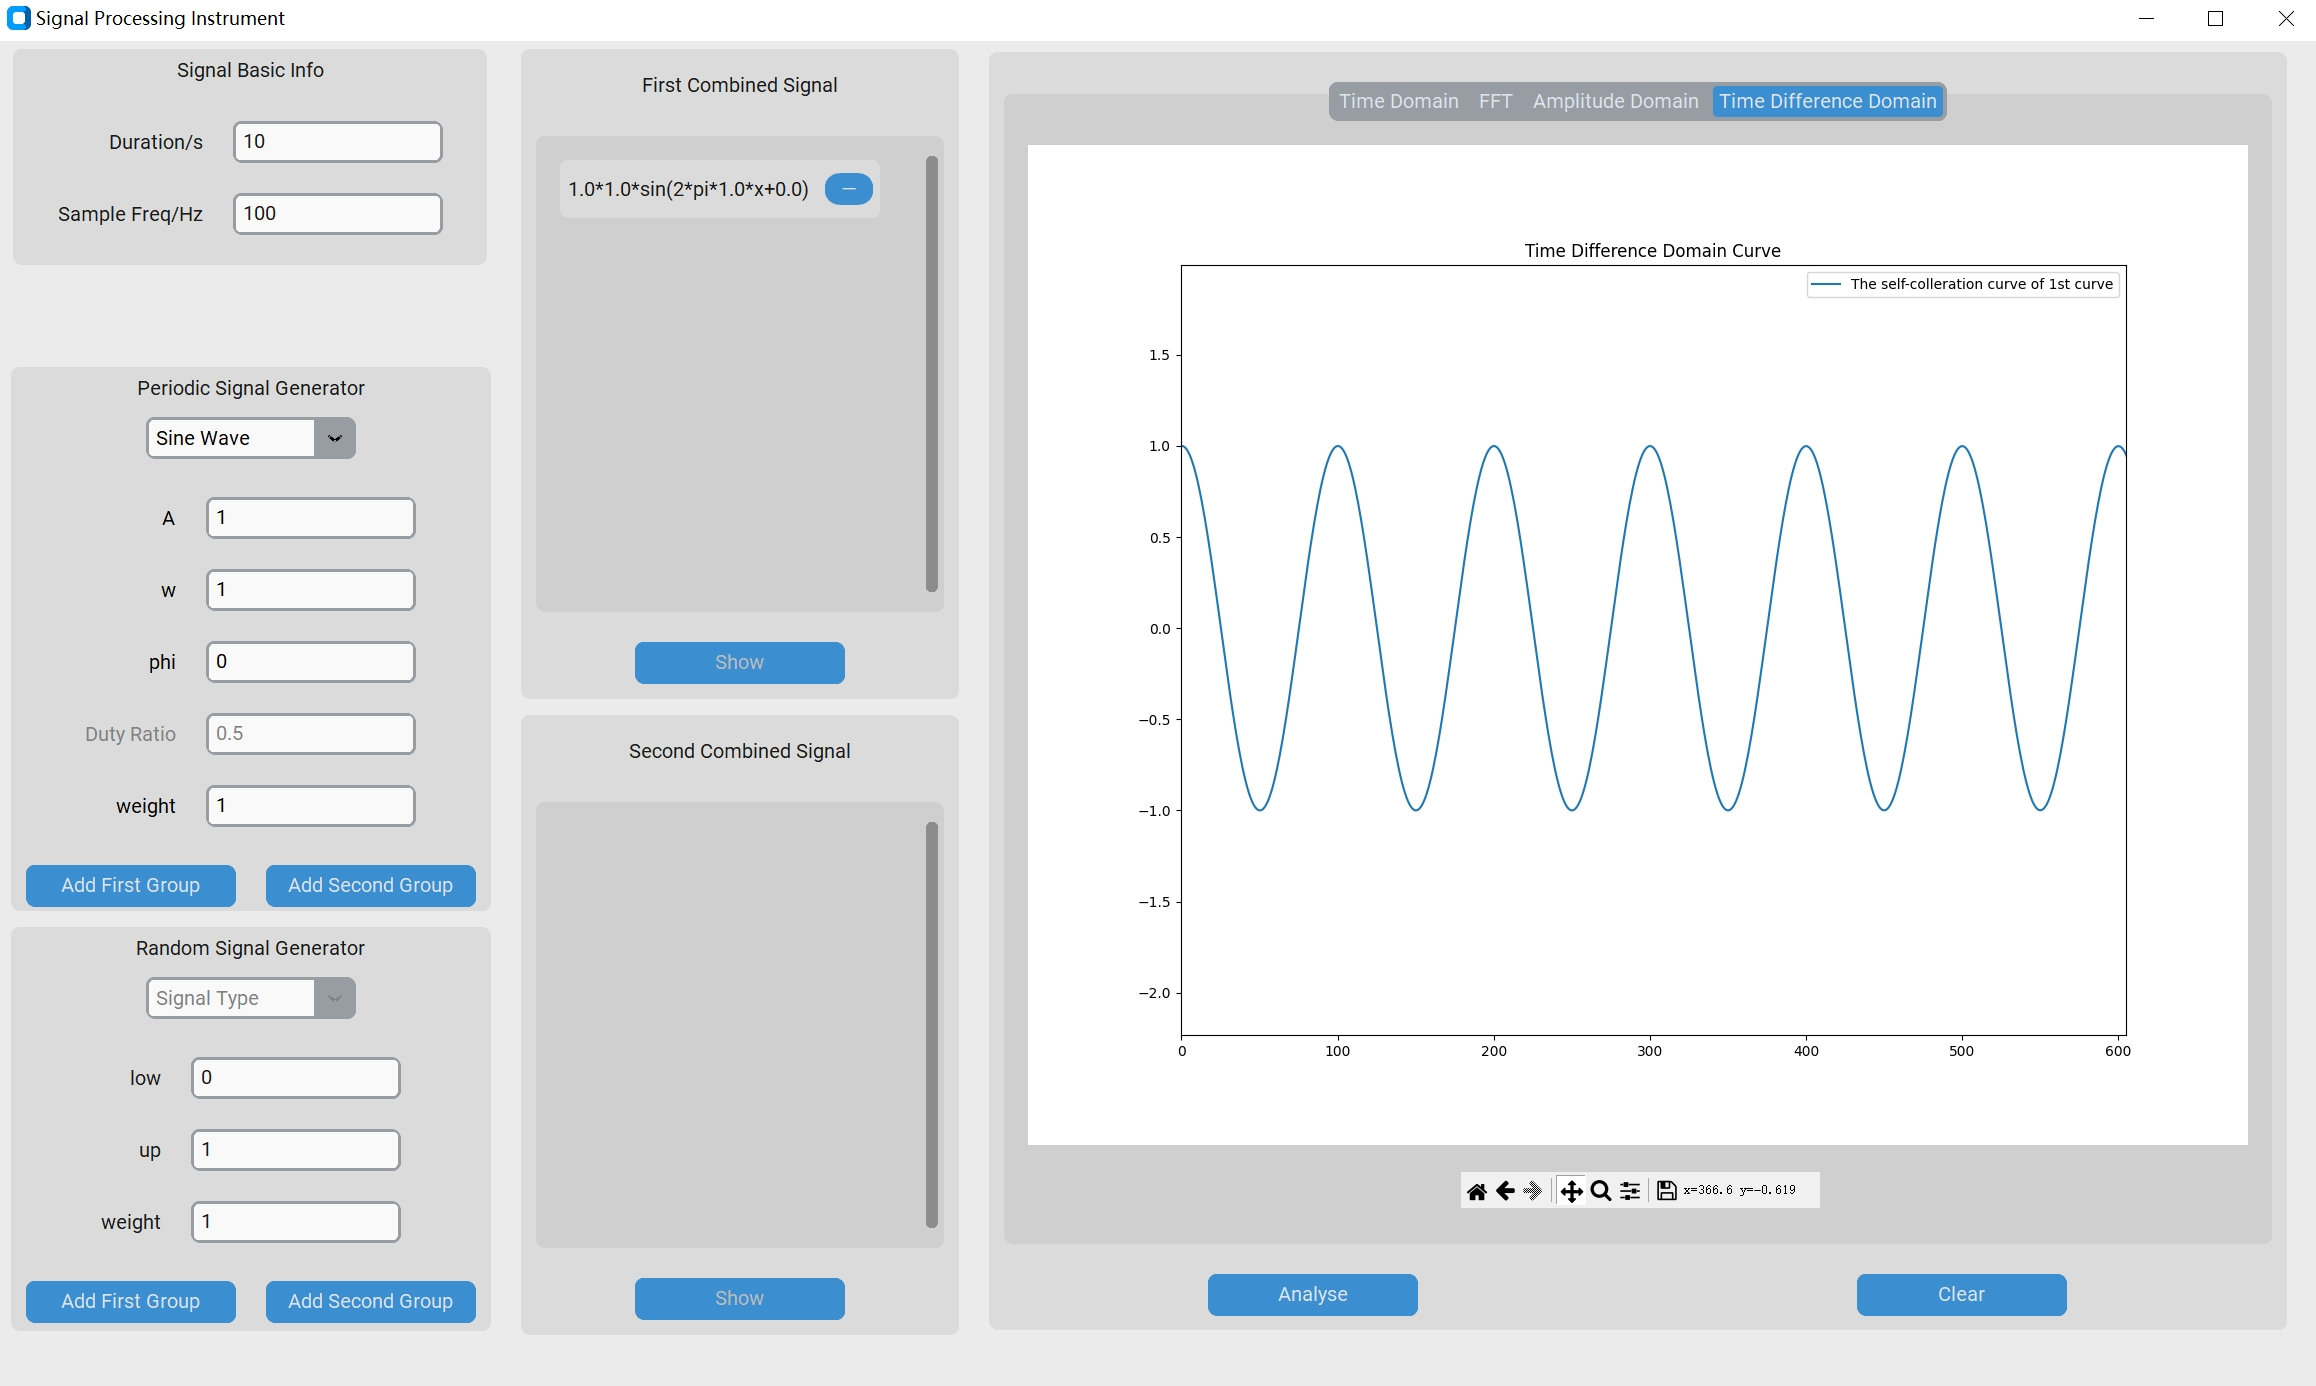
\includegraphics[width=0.9\textwidth]{img/sin_time_difference.png}
  \caption{正弦信号时差域分析结果}\label{figure6}
\end{figure}

\section{系统源码实现}

\subsection{Usage}

\begin{lstlisting}
    git clone https://github.com/dream-oyh/Control_Engneering_Twice_Work_Python.git
    cd Control_Engneering_Twice_Work_Python
    poetry install
    poetry run python main.py 
\end{lstlisting}

请确保 PC 已经安装了 poetry 和 tkinter,若未安装 poetry 包管理器,对 archlinux 用户,请运行:

\begin{lstlisting}
    sudo pacman -S python-poetry tk 
\end{lstlisting}

对 windows 用户:

\begin{lstlisting}
    pip install poetry -i https://pypi.tuna.tsinghua.edu.cn/simple
\end{lstlisting}

\subsection{后端算法程序}

\subsubsection{信号发生器}
\begin{lstlisting}[title=方波信号发生器]
def square_wave(t, augs: dict[int | float]):
  y = signal.square(2 * np.pi * augs.get("w", 0) * t, duty=augs.get('Duty Ratio',0.5))
  return y * augs.get("weight", 0)
\end{lstlisting}
\begin{lstlisting}[title=三角波信号发生器]
def triangle_wave(duration, sample_freq, augs: dict[int | float]):
    def Triangle(x: list, w, h):
        r = []
        for xi in x:
            if xi < 0.5 * w:
                r.append(2 * h * xi / w)
            else:
                r.append(-2 * h * xi / w + 2 * h / w * w)
        return r

    T = int(augs.get("T", 0))
    A = augs.get("A", 0)
    t1 = np.linspace(0, T, sample_freq * T, endpoint=False)

    y = Triangle(t1.tolist(), T, A)
    num = math.floor(duration / T) + 1
    for i in range(num):
        y = np.append(y, y)
    return y[: duration * sample_freq] * augs.get("weight", 0)
\end{lstlisting}
\begin{lstlisting}[title=正余弦信号发生器]
  def sin_wave(t, augs: dict[int | float]):
    y = (
        augs.get("weight", 0)
        * augs.get("A", 0)
        * np.sin(2 * np.pi * augs.get("w", 0) * t + augs.get("phi", 0))
    )
    return y


def cos_wave(t, augs: dict[int | float]):
    y = (
        augs.get("weight", 0)
        * augs.get("A", 0)
        * np.cos(2 * np.pi * augs.get("w", 0) * t + augs.get("phi", 0))
    )
    return y
\end{lstlisting}
\begin{lstlisting}[title=均匀分布随机信号发生器]
def uniform_wave(duration, sample_freq, augs: dict[int | float]):
    t = np.round(
        np.random.uniform(
            augs.get("low", 0), augs.get("up", 0), duration * sample_freq
        ),
        2,
    )
    return t
\end{lstlisting}
\begin{lstlisting}[title=高斯分布随机信号发生器]
  def gaussion_wave(duration, sample_freq, augs: dict[int | float]):
    t = np.round(
        np.random.normal(
            augs.get("u", 0), augs.get("sigma", 0), duration * sample_freq
        ),
        2,
    )
    return t
\end{lstlisting}
\subsubsection{信号分析算法}
\begin{lstlisting}[title=傅里叶变换]
      def fft_(self):
        first_fft = self._fft_caculate(self.first_signal)
        second_fft = self._fft_caculate(self.second_signal)
        Canvas = self.tabs.Canvas[1]
        # self.tabs.set(PROCESS_METHOD[1])
        if not isinstance(self.first_signal, int):
            self._fft_draw(
                (self.tabs.axes[1][0], self.tabs.axes[1][1]),
                self.first_t,
                first_fft,
                "1st signal",
            )
        if not isinstance(self.second_signal, int):
            self._fft_draw(
                (self.tabs.axes[1][0], self.tabs.axes[1][1]),
                self.second_t,
                second_fft,
                "2nd signal",
            )

        Canvas.draw()
\end{lstlisting}
\begin{lstlisting}[title=幅值域分析]
      def amplitude(self):
        n = 100
        list1, first_count_list = self._amplitude_analyse(self.first_signal, n)
        list2, second_count_list = self._amplitude_analyse(self.second_signal, n)
        ax = self.tabs.axes[2]
        Canvas = self.tabs.Canvas[2]
        # x_name1 = np.round(np.linspace(round(-max1, 2), round(max1, 2), n), 3).tolist()
        # x_name2 = np.round(np.linspace(round(-max2, 2), round(max2, 2), n), 3).tolist()
        x_name1 = np.round(list1, 3).tolist()
        x_name2 = np.round(list2, 3).tolist()
        x1 = range(len(first_count_list))
        x2 = range(len(second_count_list))
        if not isinstance(self.first_signal, int):
            # ax[0].bar(
            #     x=x1,
            #     height=first_count_list,
            #     label="1st signal",
            # )
            ax[0].plot(x1, first_count_list, label = "1st signal")
            ax[0].set_xticks(x1, x_name1, rotation=80)

        if not isinstance(self.second_signal, int):
            # ax[1].bar(
            #     x=x2,
            #     height=second_count_list,
            #     label="2nd signal",
            # )
            ax[1].plot(x2, second_count_list, label = "2st signal")
            ax[1].set_xticks(x2, x_name2, rotation=80)
        ax[0].legend()
        ax[1].legend()
        Canvas.draw()
\end{lstlisting}
\begin{lstlisting}[title=时差域分析]
      def colleration(self):
        ax = self.tabs.axes[3]
        Canvas = self.tabs.Canvas[3]
        # print(type(self.first_signal))
        # print(type(self.second_signal))
        if (not isinstance(self.first_signal, int)) and (
            not isinstance(self.second_signal, int)
        ):
            corr2 = self._crosscorr(self.first_signal, self.second_signal)
            ax.plot(corr2, label="The cross-correlation curve")
        elif isinstance(self.first_signal, int) and (
            not isinstance(self.second_signal, int)
        ):
            corr2 = self._autocorr(self.second_signal)
            ax.plot(corr2, label="The self-colleration curve of 2nd signal")
        elif (not isinstance(self.first_signal, int)) and isinstance(
            self.second_signal, int
        ):
            corr2 = self._autocorr(self.first_signal)
            ax.plot(corr2, label="The self-colleration curve of 1st curve")
        ax.set_xlim([0, 10])
        ax.legend()
        Canvas.draw()
\end{lstlisting}
\section{心得体会}


在开发信号发生器程序项目中,我收获了很多:

首先是对 CustomTkinter 库的深入了解,CustomTkinter 库是 Tkinter 库的扩展,可以方便地构建功能强大且美观的图形界面。通过这个项目,我学习了如何使用 CustomTkinter 库创建窗口、布局控件、处理事件等,并能够设计出美观易用的界面。利用可视化相关技术,我学习了如何使用 Matplotlib 库绘制各种类型的图形,例如波形图、频谱图、幅值图等,并能够将这些图形应用到程序中直观地呈现信号的特征。利用信号处理课程中所学知识,例如傅里叶变换、短时傅里叶变换、滤波等,我学会如何将这些知识应用到程序中实现信号的分析功能。

这个项目涉及了需求分析、系统设计、模块开发、测试与调试等多个环节。我积累了一些项目开发经验,例如如何版本管理,在 Python 的代码实现上有了进一步的认识和提高,我锻炼了自己的编程能力、信号处理能力、可视化能力和项目开发能力。我学到了如何将多种知识和技能结合起来解决实际问题,也提高了独立思考和解决问题的能力。

开发信号发生器程序项目是一个充满挑战的旅程,但也是一个收获颇丰的经历。我从中学到了很多知识,也积累了许多经验。我相信,这些收获将对我未来的学习和工作产生积极的影响。
\end{document}